\documentclass[11pt]{article}
\pdfinfoomitdate=1\pdftrailerid{}
\usepackage[letterpaper,margin=.7in,headheight=15pt,headsep=18pt,footskip=24pt]{geometry}
\usepackage[T1]{fontenc}
\usepackage{lmodern,amsmath,amssymb,array,booktabs,fancyhdr,tikz}
\renewcommand{\familydefault}{\sfdefault}
\setlength{\parindent}{0pt}\setlength{\parskip}{6pt}
\pagestyle{fancy}\fancyhf{}
\fancyhead[L]{\small Week 53 / Connecting networks / Adult return-visit guide}
\fancyfoot[L]{\scriptsize Bellingham Math Circle / Week 53 / W53-RV-FAC-v2}
\fancyfoot[R]{\thepage}
\renewcommand{\headrulewidth}{0pt}
\newcommand{\head}[1]{\par{\large\bfseries #1}\par\nobreak}
\newcommand{\sub}[1]{\par\textbf{#1}\par\nobreak}
\newcommand{\hint}[1]{\textit{Hint if needed.} #1}
\newcommand{\links}[1]{\ensuremath{\{\text{#1}\}}}
\begin{document}
\head{Mathematical overview}
\textbf{Model and first-visit facts.} Use a finite connected undirected map, whole printed links and strictly positive prices. Buying pays once per link; traveling pays for every traversal. Length on paper is not price. With every place required, a cheapest network is a tree, with $n-1$ links on $n$ places: a loop could lose a link and cost less. The first visit's other useful fact is the exchange certificate: a tree is cheapest exactly when no unused link is cheaper than a link on the tree route between its ends.

\textbf{Cheapest networks solve every lowest-dearest-route problem at once.} A route's \emph{dearest} link is its largest price, not its total. Every route along a cheapest all-place network has the smallest possible dearest price among routes with those endpoints. If a cheaper-dearest route existed, remove a dearest tree link. That separates the tree into two sides; the proposed route crosses the separation on a cheaper link, giving a cheaper tree. Conversely, a tree with this property for \emph{every} pair is cheapest, by the exchange certificate. Merely minimizing the largest price anywhere in the network is not enough.

\textbf{Opening links determines the price list and cost.} Open \emph{all} links priced at most $k$, not just a chosen network. The reachable groups only merge. Two places first share a group at exactly their lowest possible dearest price. Let $c_k$ be the number of groups and $c_0=n$. Every cheapest tree has exactly $n-c_k$ links priced at most $k$: its low-price pieces must join every group, by the preceding route fact, and each piece is a tree. Thus it has $c_{k-1}-c_k$ links of price $k$. All cheapest trees share one price list even when their links differ. For positive \emph{integer} prices,
\[
 \text{cheapest cost}=\sum_{k\ge1}k(c_{k-1}-c_k)=\sum_{k\ge0}(c_k-1).
\]
The sums stop when there is one group. Include thresholds at which nothing merges. This is an explanation of children's records, not a buying recipe to give them first.

\textbf{Trips and networks react differently to repricing.} Adding $a$ to every price adds $a(n-1)$ to every all-place tree, so it changes no cheapest network while prices stay positive. A trip of $j$ links gains $aj$, so different-length trips can overtake. Doubling preserves both kinds of optimum. More generally, strictly increasing repricing preserves all cheapest all-place trees, including ties, because it preserves every exchange comparison. Squaring positive prices can nevertheless change cheapest trips.

\textbf{Optional places change the problem.} Circles must connect; squares need not. A cheapest purchase has no loop and no optional leaf: either could be trimmed for a saving. With two required places it is a cheapest trip; with all places required it is the original tree problem. In between, a purchase can resist every cheaper single change yet not be cheapest. With $r\ge2$ required places, at most $r-2$ optional places can have three or more bought links; the leaf-count proof is on guide p.~\pageref{leaf}. The all-place route, price-list, cost-from-groups, repricing and converse claims do \emph{not} extend to optional places.

\textbf{Discovery and evidence.} K--1 should notice when two places first join a group and that a square can save, tie or cost extra (dots to 4, totals to 12). Grades 2--3 should connect the lowest dearest price to the first common ring, and notice that adding to every price can switch a trip while keeping the network (printed totals to 18). Grades 4--5 should explain these patterns by cuts and equal link counts, then test their limits with squares. A pattern seen on one map is a \emph{conjecture}; a complete catalog proves that case, while cut and leaf arguments explain general claims. Incomplete searching proves no impossibility. Adults may read and record; children choose the links.
\newpage
\head{Preparation and shared launch}
\textbf{Status.} Unpiloted and physically unrehearsed. Print scale, tape clearance, pawn fit, counter handling, preparation time and the proposed pacing still need a real rehearsal. Digital checks do not establish classroom readiness.

\textbf{Kits and prints.} Each pair or grades 4--5 trio reuses 30 counters (12--15 mm), ten removable tape strips ($5\times20$ mm), a pawn or finger, a sleeve/pen for erasable rings, a tray and scrap paper for a second payment area. Two K--1 kits, two grades 2--3 kits, one grades 4--5 kit, plus 15 demonstration counters and four strips: \textbf{165 counters and 54 strips}. These are planning quantities, not attendance.

Print selected student pages once per pair/trio: \texttt{k-1.pdf} (7 pages), \texttt{grades-2-3.pdf} (6), \texttt{grades-4-5.pdf} (10), US Letter, single-sided, 100\%. Cut nothing. Large maps are mats; small records/examples are pen-only. Working circles are 10 mm across, centers at least about 40 mm apart. No base page is needed; optionally print base \texttt{week-53-students.pdf} p.~3 (trap). There is no base materials PDF. Base guide: W53-guide-v4.

Most K--1 children are new: teach buying/paying. Many grades 2--3 children met only base pp.~1--4; do not assume swaps. Repeats: K--1 P1 is base P2; grades 4--5 P4 is base P4; grades 2--3 P5 and grades 4--5 P8/P9-bottom reuse base P6/P8's six-place map. Expect remembered answers; rings, price lists and trips are new questions.

Allow an unmeasured 15--20 minutes for prints/kits. Test strips on the six-place grid (grades 2--3 p.~4 or grades 4--5 p.~7), keeping prices visible and counters off roads; use a finger if a pawn hides a place. Write oversized trial totals, including the squared price 36. The kit covers optimal single payments, not every purchase: $18+15=33$ and $16+16=32$, so record one total and reuse its counters.

\textbf{Whole group, 5 minutes including free handling.} On the board use this non-task line (circles about 10 mm, centers at least 40 mm apart). Let a child mark one whole link and pay, then finish the line.
\begin{center}
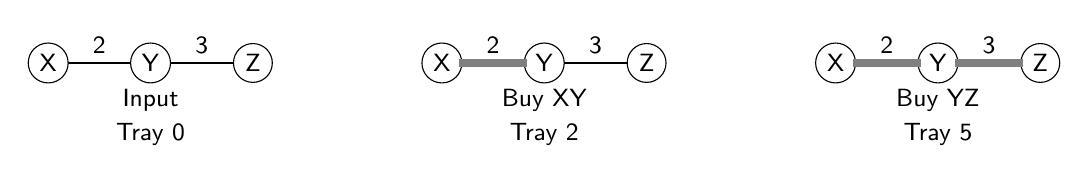
\begin{tikzpicture}[x=1cm,y=1cm, every node/.style={font=\small}]
\foreach \offset/\caption in {0/Input,5/Buy XY,10/Buy YZ}{
 \begin{scope}[xshift=\offset cm]
 \draw (0,0)--(1.3,0)--(2.6,0);
 \node[above] at (.65,0){2}; \node[above] at (1.95,0){3};
 \foreach \x/\s in {0/X,1.3/Y,2.6/Z}{\node[circle,draw,fill=white,inner sep=2pt] at (\x,0){\s};}
 \node at (1.3,-.48){\caption};
 \end{scope}}
 \draw[line width=3pt,gray] (5.22,0)--(6.08,0);
 \draw[line width=3pt,gray] (10.22,0)--(11.08,0) (11.52,0)--(12.38,0);
 \node at (1.3,-.9){Tray 0};\node at (6.3,-.9){Tray 2};\node at (11.3,-.9){Tray 5};
\end{tikzpicture}
\end{center}
Say: ``A network lets the pawn walk between every circled place on bought roads. On your maps, try to pay as few counters as you can. Trace X--Y--Z again without paying; then return a link and refund it. At each table demonstrate its next convention using the printed start/step/result: opening (K--1 p.~2; grades 2--3 p.~2; grades 4--5 p.~3), trips (grades 2--3 p.~3; grades 4--5 p.~6), or squares (K--1 p.~4; grades 2--3 p.~6; grades 4--5 p.~8). A trip uses all printed roads: write its word, then pay (XYZ costs 5; XYZY costs 8). Squares may be passed through but need not be visited. Introduce these separately.

\textbf{Staffing and one hour.} One adult per table; parent volunteer at K--1. Read K--1 P2 and grades 2--3 P3 pointing to pictures; K--1 children identify groups, adults may ring tiny records. Pool six-network catalogs; spare maps are workspace. Paraphrase grades 4--5 P10's ``change'' and Lee's P12 claim. The trio rotates chooser, payer/checker, recorder. Adults read/record, children choose.

Use 5 minutes movement, 5 handling/launch, 20 exploring, 5 break, 20 continuing, 5 sharing. \textbf{K--1: P1, P2, P4}, then P3 or P5; later visit P5--6, then P7--8 if ready. \textbf{Grades 2--3: P1--3}, then P4; later visit P5--8. \textbf{Grades 4--5: P1, P3, P7}, then P9 or P10; pool P2 or save it with P4. P5--6/P11--12 offer later explanations. Finishing every page is not the goal.
\newpage
\head{K--1 solutions and discretionary hints}
AB means the whole link; buying it first or last does not make a new network. Spare record maps are workspace, not a promise of that many answers. Let children choose; the adult can read, count and draw their chosen links.

\sub{Problem 1 page 1}
Minimum \textbf{4}, exactly \links{AB, AC, CD}, \links{AB, BC, CD}, \links{AC, BC, CD}. Reaching D costs at least 2, and two more links at least 1 each. Equality requires CD and two triangle sides; all three pairs work. \hint{``Which road could reach D? Could the same payment buy a different triangle pair?''}

\sub{Problem 2 page 2}
With 1-dot links open, groups are \textbf{AB / C / D / EF}; up to 2 dots, \textbf{ABC / DEF}; up to 3 dots, \textbf{ABCDEF}; up to 4 dots, still one group. The pawn first reaches F from A at \textbf{3}. Include isolated places in rings. Opening means marking every eligible link; no payment total is requested. \hint{``Where can the pawn go without crossing an unmarked road?''} A group need not look round; its membership matters.

\sub{Problem 3 page 3}
Minimum \textbf{9}: \links{AB, AC, CD, DE, EF} or \links{AB, BC, CD, DE, EF}. Price list $1,1,2,2,3$: AB/EF are forced cheapest exits; DE joins D/E; AC or BC joins C; CD is the cheapest crossing between ABC and DEF. Without 3- or 4-dot links those groups stay apart. \hint{``Can you cross between the rings without a 3 or 4?''}

\sub{Problems 4 and 5 pages 4 and 5}\label{starforms}
Each outer triangle has three links priced 4. Without S, any two cost \textbf{8}, the minimum. For P4, using S costs \textbf{6}, uniquely AS, BS, CS. For P5's top map, using S costs \textbf{9}, uniquely the three spokes: the square costs one extra. On P5's bottom map, using S costs \textbf{8}: AS, BS together with \emph{one of} CS, AC or BC. The square ties rather than saves. Those are all three cheapest ways using S; adding the three outer pairs gives six cheapest overall.

Why complete: a cheapest join using S is a tree with three spokes, two spokes plus one outer link, or one spoke plus two outer links. Compare these forms, retaining the last even though it is wasteful when S is optional. \hint{P4: ``Must every circle use an outside road?'' P5: ``Must using the square mean buying all its roads?''} Keep both payment piles.

\sub{Problem 6 page 6}
Without X: \textbf{12}, any three outer sides (four choices). Using X: \textbf{8}, uniquely AX, BX, CX, DX. Three outer links cost 12; a five-place tree needs four links, each at least 2, and the four spokes attain 8. \hint{``Could any other four-link purchase cost 8?''}

\bigskip
\head{K--1 continuation and grades 2--3 entry}
\sub{K--1 Problem 7 page 7}\label{two-squares}
Minimum \textbf{6}, uniquely AS, BS, ST, CT, DT. Neither square: 10 (AB, AC, CD); only S or only T: 9. With both, five links are needed, but only four price-1 links exist: $1+1+1+1+2=6$. \hint{``How can the two small groups join through their squares?''} A readiness-dependent continuation.

\sub{K--1 Problem 8 page 7}
Use positive whole-number dots. A working answer is \textbf{2, 2, 4} on the three spokes; 1, 3, 4 and 2, 3, 3 also work, in any arrangement. Complete rule: sort the spoke prices $x\le y\le z$. The cheapest join using S costs $\min(x+y+z,x+y+4,x+8)$. It equals 8 exactly for \textbf{$(1,3,z)$ or $(2,2,z)$ with $z\ge4$, or $(2,3,3)$}. Do not cap invented dots unless reducing the task deliberately. \hint{``Could two square roads and one outside road beat your three roads?''} A sum of 8 alone fails: 1, 1, 6 has a cost-6 alternative. The printed prompt leaves positivity implicit; say ``at least one dot per road'' before inventing prices.
\head{Grades 2--3 solutions and discretionary hints}
\sub{Problem 1 page 1}\label{six-networks}
Minimum \textbf{9}. Every cheapest network uses CD and EF, any two of AB, AC, BC, and one of CE, DE. The complete six are:
\begin{center}\small
\begin{tabular}{ll}
AB, AC, CD, CE, EF & AB, AC, CD, DE, EF\\
AB, BC, CD, CE, EF & AB, BC, CD, DE, EF\\
AC, BC, CD, CE, EF & AC, BC, CD, DE, EF
\end{tabular}
\end{center}
A tree needs five links. The three usable price-1 links join ABC/EF; CD is D's cheapest exit; crossing ABCD/EF costs at least 4. Equality gives exactly the $3\times2$ listed choices. \hint{``Which part is still separate? If you keep the right side the same, how many ways can you join A, B and C?''}

\sub{Problems 2 and 3 pages 1 and 2}\label{routes-groups}
\begin{center}\small
\begin{tabular}{llll}
Pair & One lowest-dearest route & Dearest price & First common ring\\\midrule
A to D & ACD & 2 & 2\\
B to D & BCD & 2 & 2\\
D to F & DEF & 4 & 4\\
A to F & ACEF & 4 & 4
\end{tabular}
\end{center}
Other routes can be equally good; these problems do not request all routes. For P3: at price 1 the groups are \textbf{ABC / D / EF}; at 2, \textbf{ABCD / EF}; at 3, unchanged; at 4, one group. D is isolated below 2, and EF is separate below 4, proving the lower bounds. \hint{P2: ``Are we adding the prices or choosing the biggest?'' P3: ``Did the price-3 road actually join different groups?''}

\bigskip
\head{Grades 2--3 trips and optional places}
\sub{Problem 4 page 3}\label{trip-key}
On all three maps the cheapest network is AB, BC, CD. Their costs are \textbf{3, 6, 9} for original, +1 and +2 prices. Cheapest A--D trips are respectively \textbf{ABCD at 3; AD at 5; AD at 6}, each unique. These are the only two simple A--D routes; a repeated part costs extra. \hint{``Which roads stayed the same even though their total changed?''} Record links as well as costs, using the printed lines.

\sub{Problem 5 page 4}\label{grid-key}
On all three maps the cheapest network is \textbf{AB, BC, CD, DE, EF}. Complete trip key:
\begin{center}\small
\begin{tabular}{llll}
Prices & Network cost & Every cheapest A--F trip & Trip cost\\\midrule
Original & 8 & ABCDEF, ACDEF & 8 each\\
Every price 2 more & 18 & ACDF & 15\\
Doubled & 16 & ABCDEF, ACDEF & 16 each
\end{tabular}
\end{center}
For the network, AB, BC, CD, DE, EF are uniquely cheapest across cuts A / rest, AB / rest, ABC / DEF, ABCD / EF and ABCDE / F respectively. For trips, both original ways to reach C cost 3; then CDE costs 3 and EF costs 2. After +2, AC wins to C and DF wins from D to F. Guide p.~\pageref{trip-certificate} gives a complete shortest-trip certificate. \hint{``Can a road we did not buy still be used on a trip?''} Yes: a trip is on the whole printed map.

\sub{Problems 6 and 7 page 5}
P6: write AB$=a$, BC$=b$, AC$=c$, using positive whole numbers. For a \emph{strict} switch, $a+b<c<a+b+2$, hence \textbf{$c=a+b+1$}. For example 1, 1, 3; 1, 2, 4; 2, 2, 5. The two-link trip gains 4 while the direct trip gains 2. \hint{``How much did each trip gain?''} If a child allows tied cheapest trips, $a+b\le c\le a+b+2$ also meets a weak reading of the prompt; ask whether they intended a tie or a clear switch, rather than rejecting it.

P7: \textbf{No; no}, for the no-square maps used so far and changes keeping prices positive. Every connecting tree has the same number of links, so adding the same amount preserves its ranking; doubling doubles every trip total. \hint{``Do all networks gain the same number of extra counters? Do all trips?''} P8 changes the rules, so the first answer need not survive there.

\sub{Problem 8 page 6}
Left: \textbf{8 without S, 6 using S}. Right: \textbf{8 without, 9 using}. Without, choose any two outer links; using, the unique minimum is AS, BS, CS on each map. The three tree forms on guide p.~\pageref{starforms} prove the comparisons. \hint{``Is an optional place always a bargain?''} Let the child demonstrate the two piles before discussing a general rule.
\bigskip
\head{Grades 4--5: routes, groups and general claims}
\sub{Problem 1 page 1}
Use the complete grades 2--3 P2 key (guide p.~\pageref{routes-groups}), including its lower bounds. \hint{``Which groups remain apart if that largest price is forbidden?''}

\sub{Problem 2 page 2}
Use grades 2--3 P1's complete six-network key and proof (guide p.~\pageref{six-networks}), minimum \textbf{9}. \hint{``Which links occur in every network? Where do they differ?''} Pool cases; spare records here and in P4 are workspace.

\sub{Problem 3 page 3}
Use grades 2--3 P3's groups and first-common thresholds (guide p.~\pageref{routes-groups}). Including the six isolated places before any link opens gives $c_0,\ldots,c_4=\mathbf{6,3,2,2,1}$. \hint{``If a road opens inside one ring, does the number of groups change?''}

\sub{Problem 4 page 4}
Minimum \textbf{6}, exactly \links{AB, AC, CD, DE}, \links{AB, BC, CD, DE}, \links{AC, BC, CD, DE}. Groups: at 1, \textbf{ABC / D / E}; at 2, \textbf{ABCDE}, unchanged thereafter. All optima have prices \textbf{1,1,2,2}: a four-link tree can use only two price-1 triangle sides, so costs at least 6; equality needs CD, DE and a triangle pair. \hint{``Do three price-1 links help reach D or E?''}

\sub{Problem 5 page 5}
\textbf{Sam is wrong.} All four trees have largest price 3, but BC, CD, AD costs \textbf{9}; the other three cost \textbf{7} (AB and any two other sides). The unavoidable largest price does not determine total. \hint{``Same dearest road, different payment piles?''} Sam checks one number; P6 checks every pair.

\sub{Problem 6 page 5}
\textbf{Yes; no; yes}, on a connected positive-price map with no squares. Every cheapest-network route is lowest-dearest; all cheapest networks have the same price list; threshold groups determine cost. The proof ideas open this guide. Two examples suggest, but do not prove, a universal statement.

For P2--3 the group drops are $6-3=3$, $3-2=1$, $2-2=0$, $2-1=1$. Therefore there are \textbf{three price-1 links, one price-2 and one price-4}, giving $3+2+4=9$. Alternatively add $5+2+1+1=9$. For P4, the drops are $5-3=2$, $3-1=2$, giving $2+4=6$, or $(5-1)+(3-1)=6$. Count the threshold-3 pause in the first map even though no link of that price is bought.

\hint{``Suppose a cheaper-dearest route existed. What happens if we lift the dearest road in your tree?''} Draw the two resulting sides and let the child find where the proposed route crosses. For the price-list question ask, ``How many links are needed inside each ring?'' Save the converse for P12.

\textbf{Limit.} P9's 2,2,4-spoke map has cheapest lists 4,4 and 2,2,4: optional squares change the theorem.
\bigskip
\head{Grades 4--5 trips and optional places}
\sub{Problem 7 page 6}
Use grades 2--3 P4's complete network/trip key (guide p.~\pageref{trip-key}). \hint{``Which payment counts every bought road, and which counts only your trip?''} Reuse the printed trip example before comparing totals.

\sub{Problem 8 page 7}
Every cheapest network is \textbf{AB, BC, CD, DE, EF}, uniquely. The grades 2--3 P5 cut argument proves this. For the original, +2 and doubled rows, use its complete key (guide p.~\pageref{grid-key}); the additional squared row is below.
\begin{center}\small
\begin{tabular}{llll}
Prices & Network cost & Every cheapest A--F trip & Trip cost\\\midrule
Each price times itself & 14 & ABCDEF & 14
\end{tabular}
\end{center}
\textbf{Complete trip certificate.}\label{trip-certificate} The least costs from A to A,B,C,D,E,F are respectively
\[
\begin{array}{c|rrrrrr}
 &A&B&C&D&E&F\\\hline
\text{original}&0&1&3&5&6&8\\
+2&0&3&5&9&12&15\\
\times2&0&2&6&10&12&16\\
\text{squared}&0&1&5&9&10&14
\end{array}
\]
Every printed link satisfies $d(v)\le d(u)+w(uv)$ in both directions; summing along a route proves its cost is at least the destination label. The listed trips attain the bound. Equality requires each step to advance by exactly its price: originally C can follow either A or B, while D, E, F must follow C, D, E; after +2 the successful chain is A,C,D,F; doubling keeps the original choices; squaring forces A,B,C,D,E,F. Thus no cheapest trip is missing. These adult labels are not an extra child ledger.

None of the three changes alters cheapest \emph{all-place} networks. Addition and squaring can change cheapest trips; doubling cannot. \hint{``What does adding 2 do to a three-road trip compared with a five-road trip?''} For squaring ask which costly single road now competes with several cheaper ones. A change that can alter the cheapest network is $p\mapsto7-p$: its minimum is 15, and AB, BC, CD, DE, EF is no longer cheapest. Price order matters.

\sub{Problem 9 page 8}
\textbf{Left star: cost 8, three ways}, AB/AC, AB/BC, AC/BC; S is unused. A tree using S costs at least 9. \textbf{Right star: cost 8, six ways}: those same three outer pairs, plus \links{AS, BS, CS}, \links{AS, BS, AC}, \links{AS, BS, BC}. The three tree forms from guide p.~3 show completeness. \textbf{Bottom map: cost 8, two ways}, \links{AB, BC, CD, DE, EF} and \links{AC, CD, DE, EF}. Only A and F are circles; B,C,D,E are squares. A positive-price optimum for two required endpoints is just a cheapest simple trip, so P8's original trip list proves completeness. \hint{``Which places must be reached here? Could you return a road that goes only to an optional dead end?''}

\sub{Problem 10 page 9}
Cheapest is \textbf{6}, uniquely AS, BS, CS. From AB and BC, the answer is \textbf{no}: with a cap of 8, a purchase with no spoke can only be an outer pair. Returning a link disconnects a circle; buying any link exceeds 8; swapping an outer link for one spoke still disconnects a circle. Only swaps to the other outer pairs survive. The same holds with cap 9. A cap of \textbf{10} is enough: buy AS (10), swap AB for BS (8), swap BC for CS (6). \hint{``Could one new spoke connect both sides left by returning an outside road?''} A swap is one atomic exchange; its final state must connect the circles. This optional-place example, not a contradiction, marks the limit of the first-visit exchange test.
\newpage
\head{Grades 4--5 continuations, explanations and sources}
\sub{Problem 11 page 10}\label{leaf}
Minimum \textbf{6}, uniquely AS, BS, ST, CT, DT, as in K--1 P7 (guide p.~\pageref{two-squares}). A square place cannot have just one bought link in an unrestricted cheapest purchase: that link is a positive-price dead end, removable without separating any required circle. A square can be unused (degree zero); do not confuse that with an optional leaf in the bought tree.

With four circles, at most \textbf{2} squares can have three or more bought links; S and T attain it. Generally ignore unused places. The bought tree has only required leaves. If there are $L$ leaves and branch degrees $d_i\ge3$, counting link ends gives
\[
-L+\sum_i(d_i-2)=-2,\qquad L=2+\sum_i(d_i-2).
\]
Degree-2 places contribute zero; each branch contributes at least one. Hence at most $L-2\le r-2$ branches when $r\ge2$ places are required. With $r=4$, at most two are optional branches. \hint{``When a path splits, how many extra ends must appear?''} Drawn branches can explain the bound; this map alone proves only attainability.

\sub{Problem 12 page 10}
\textbf{Lee is right}, on a connected positive-price map with no squares. First test P5's cost-9 purchase BC, CD, DA: its A--D--C--B route has dearest price 3, but AB costs 1, so it fails Lee's test. Sam's one number for the whole network misses this contrast.

Each unused link $f$ is itself an available route, so Lee's condition says $f$ costs at least every link on the tree route between its ends. This is the base week's exchange certificate, which proves global cheapestness; see W53-guide-v4, p.~7 for the transformation proof. \hint{``What does Lee's condition say about a route consisting of just one unused road?''} Enact one exchange before returning to the general explanation.

\sub{Sources consulted and boundaries}
{\small
Reviser checked the final student PDFs W53-RV-K/M/U-v1, outline, draft, reviews and base guide W53-guide-v4 (exchange proof p.~7). The writer also consulted student sources, base research notes, Week 8 return-visit and Week 98 model guides. Use final-PDF numbering, not old page-review numbering.

The outline's background, not newly consulted originals: lowest-dearest routes (grades 2--3 P2--3; grades 4--5 P1/P3/P6) from Hu, ``The Maximum Capacity Route Problem,'' \textit{Operations Research} 9(6), 1961, pp.~898--900 (outline author checked abstract only), and Wikipedia's ``Widest path problem''; repricing (grades 2--3 P7; grades 4--5 P8) from Sedgewick/Wayne, \textit{Algorithms}, 4th ed., \S4.3 companion, Exercise 1; Sam (grades 4--5 P5) from its Web Exercise 1; squares (grades 4--5 P9--11) from ``Steiner tree problem.'' Hwang/Richards/Winter, \textit{The Steiner Tree Problem} (1992), is cited background, not consulted.

Base notes trace the activity to CS Unplugged Activity 9, ``The Muddy City,'' printed pp.~76--80/PDF pp.~1--5, and \textit{Math Circle by the Bay}, ``How we teach,'' p.~ix/PDF p.~10. Those originals were unavailable. Elementary proofs and finite checks are supplied here. Materials and pacing remain untested; record actual use and handling issues.
}
\end{document}
